\documentclass[conference]{IEEEtran}
\usepackage{cite}
\usepackage{amsmath}
\usepackage{graphicx}
\usepackage{booktabs}
\usepackage{url}
\usepackage{tikz}
\usetikzlibrary{arrows.meta,positioning,fit}
\usepackage{microtype}
\def\BibTeX{{\rm B\kern-.05em{\sc i\kern-.025em b}\kern-.08em T\kern-.1667em\lower.7ex\hbox{E}\kern-.125em X}}

\begin{document}

\title{Production-Ready MLOps Pipeline for Smartphone-Based Sprint Biomechanics: From Research Prototype to Scalable Coaching Platform}

\author{\IEEEauthorblockN{Y.~Teja, Shaik Sadiya Anmol, Varsha~R, Yeshitha~P}
\IEEEauthorblockA{Department of CSE-AIML, Dayananda Sagar University\\
Email: tejachey75@gmail.com}
\and
\IEEEauthorblockN{Dr.~Bahubali Shiragapur}
\IEEEauthorblockA{Department of CSE-AIML, Dayananda Sagar University\\
Email: bhahubali-aiml@dsu.edu.in}
\and
\IEEEauthorblockN{Dr.~Puneeth~N}
\IEEEauthorblockA{Department of AI \& Robotics, Dayananda Sagar University\\
Email: puneethn-air@dsu.edu.in}}

\maketitle

\begin{abstract}
Laboratory motion capture for sprint biomechanics costs USD~100k--500k, which puts it out of reach for most athletes. We present a reproducible, containerised MLOps pipeline that combines a single 60\,fps smartphone video (MediaPipe Pose) with a Galaxy Watch4 Classic IMU (100\,Hz) to extract 19 sprint features. Performance labels come from an objective, automatically measured quantity, the athlete's body-size-normalised running velocity, instead of subjective ratings. Video--IMU integration is validated quantitatively: stride frequency from the two sensors agrees with a mean absolute error of 0.07\,Hz ($r=0.95$), and automatic clock and cadence checks flagged two of nine watch files that did not belong to the filmed sprint. A request takes a median 2.1\,s end to end, the service sustains about 1.2 clips/s on one 10-core node with no failed request in 214, and recovers from a worker or server-process crash in about one second or less. In a leakage-free leave-one-subject-out pilot with eight athletes (nine trials), three-tier classification did not exceed chance with statistical significance (best 55.6\%, $p=0.16$); earlier reported accuracies came from label circularity and augmentation leakage, which we document. A power analysis shows that drift alarms need at least 100 reference recordings, so the system arms them only above that size and gates every model with a promotion test.
\end{abstract}

\begin{IEEEkeywords}
sprint biomechanics, MLOps, pose estimation, wearable IMU, drift detection, model registry
\end{IEEEkeywords}

\section{Introduction}
Sprint speed depends on stride frequency, ground contact time and joint kinematics, and measuring them lets coaches find inefficiencies and asymmetries~\cite{weyand2000}. Optical motion capture is accurate but expensive and confined to laboratories~\cite{colyer2018}. Markerless pose estimators such as MediaPipe/BlazePose~\cite{bazarevsky2020} and OpenPose~\cite{cao2021} run on commodity hardware and single-camera video can approximate laboratory gait measures~\cite{kidzinski2020}, while consumer smartwatches add inertial signals. Turning such a prototype into a service raises engineering questions that accuracy alone does not answer: are the two sensors really synchronised, are results reproducible, is a retrained model safe to deploy, and what happens when the data change~\cite{sculley2015}?

This paper reports an MLOps pipeline for smartphone video plus smartwatch IMU sprint analysis and, as importantly, an honest evaluation of it. Its contributions are:
\begin{enumerate}
\item an objective, annotation-free performance label (normalised running velocity) and a data-quality gate that quarantines mismatched sensor files automatically (Sections~\ref{sec:data}--\ref{sec:integration});
\item a versioned, containerised pipeline with experiment tracking, a promotion-gated model registry, a drift monitor and a retraining loop (Section~\ref{sec:mlops});
\item a leakage-free, subject-independent evaluation that corrects accuracies reported in an earlier version of this work (Section~\ref{sec:results});
\item measured latency, throughput, fault-tolerance and drift-detection evidence (Sections~\ref{sec:latency}--\ref{sec:ops}).
\end{enumerate}

\section{Related Work}
\emph{Markerless motion analysis.} Vision-based systems are replacing marker-based capture in sport~\cite{colyer2018}; lightweight estimators such as BlazePose~\cite{bazarevsky2020} and OpenPose~\cite{cao2021} run in real time on commodity hardware, and single-camera deep-learning pipelines recover clinically relevant gait parameters~\cite{kidzinski2020}. Most such studies examine walking, not maximal-effort sprinting, where motion blur and speed stress the estimators.
\emph{Sprint biomechanics.} Top running speed is set by the force applied to the ground rather than by leg-swing rate~\cite{weyand2000}, which is why ground contact time and step frequency are the key features here and why a wrist-worn IMU, which senses arm swing and trunk impact, is only an indirect proxy.
\emph{MLOps and monitoring.} Machine-learning systems accumulate hidden technical debt in data dependencies, configuration and feedback loops~\cite{sculley2015}; experiment tracking and model registries~\cite{zaharia2018} and concept-drift handling~\cite{gama2014} are standard remedies, but they are rarely evaluated on small, sensor-heterogeneous sports data, which is the gap this paper addresses.

\section{Data and Labels}\label{sec:data}
\subsection{Dataset}
Nine maximal-effort fly sprints were recorded from \emph{eight} athletes (one athlete ran two trials) in a single outdoor session on a synthetic track. All participants gave informed consent, and participant details are confidential and not reported. Video was recorded with a tripod-mounted smartphone at 1920$\times$1080, 60\,fps (HEVC), camera orthogonal to the running direction; athletes crossed the field of view in 0.9--1.7\,s. A Samsung Galaxy Watch4 Classic worn on the left wrist recorded triaxial acceleration and angular velocity at a measured 99.3--99.6\,Hz with the Sensor Logger application. The raw recordings cannot be released because of the consent given; the code, parameters, tests and container definition are public.\footnote{\url{https://github.com/TejaChey/Multimodal_AI_Based_Motion_Analysis}}
The dataset is small: eight athletes and nine trials limit every claim in this paper, and we therefore present the classification study as a pilot (Section~\ref{sec:limits}).

\subsection{Objective performance labels}\label{sec:labels}
An earlier version of this work labelled athletes by clustering the same features later used for classification, which is circular, and described the labels as expert ratings. We replace them with a measured quantity that is \emph{not} a model input: the athlete's horizontal velocity. The mid-hip landmark position is regressed on time with a Theil--Sen estimator~\cite{sen1968} ($R^2\geq0.998$ for all nine recordings), and the pixel velocity is divided by a posture-invariant body length $L$ (trunk + thigh + shank, median over frames), which equals $0.779\times$ stature~\cite{drillis1966}. This gives velocity in statures per second, independent of camera distance (verified in unit tests at 120 and 300\,px stature). Assuming a 1.70\,m stature, velocities range from 6.7 to 9.4\,m/s (mean 7.7). Tiers are cohort tertiles (Beginner / Intermediate / Elite); both trials of the repeated athlete fall in the same tier (Fig.~\ref{fig:labels}). Labels are measured automatically, so new recordings need no annotator. Only frames of the sprinting athlete are used: MediaPipe occasionally locks onto a static false detection, and we keep the continuous track with the largest horizontal travel.

\begin{figure}[t]
\centering
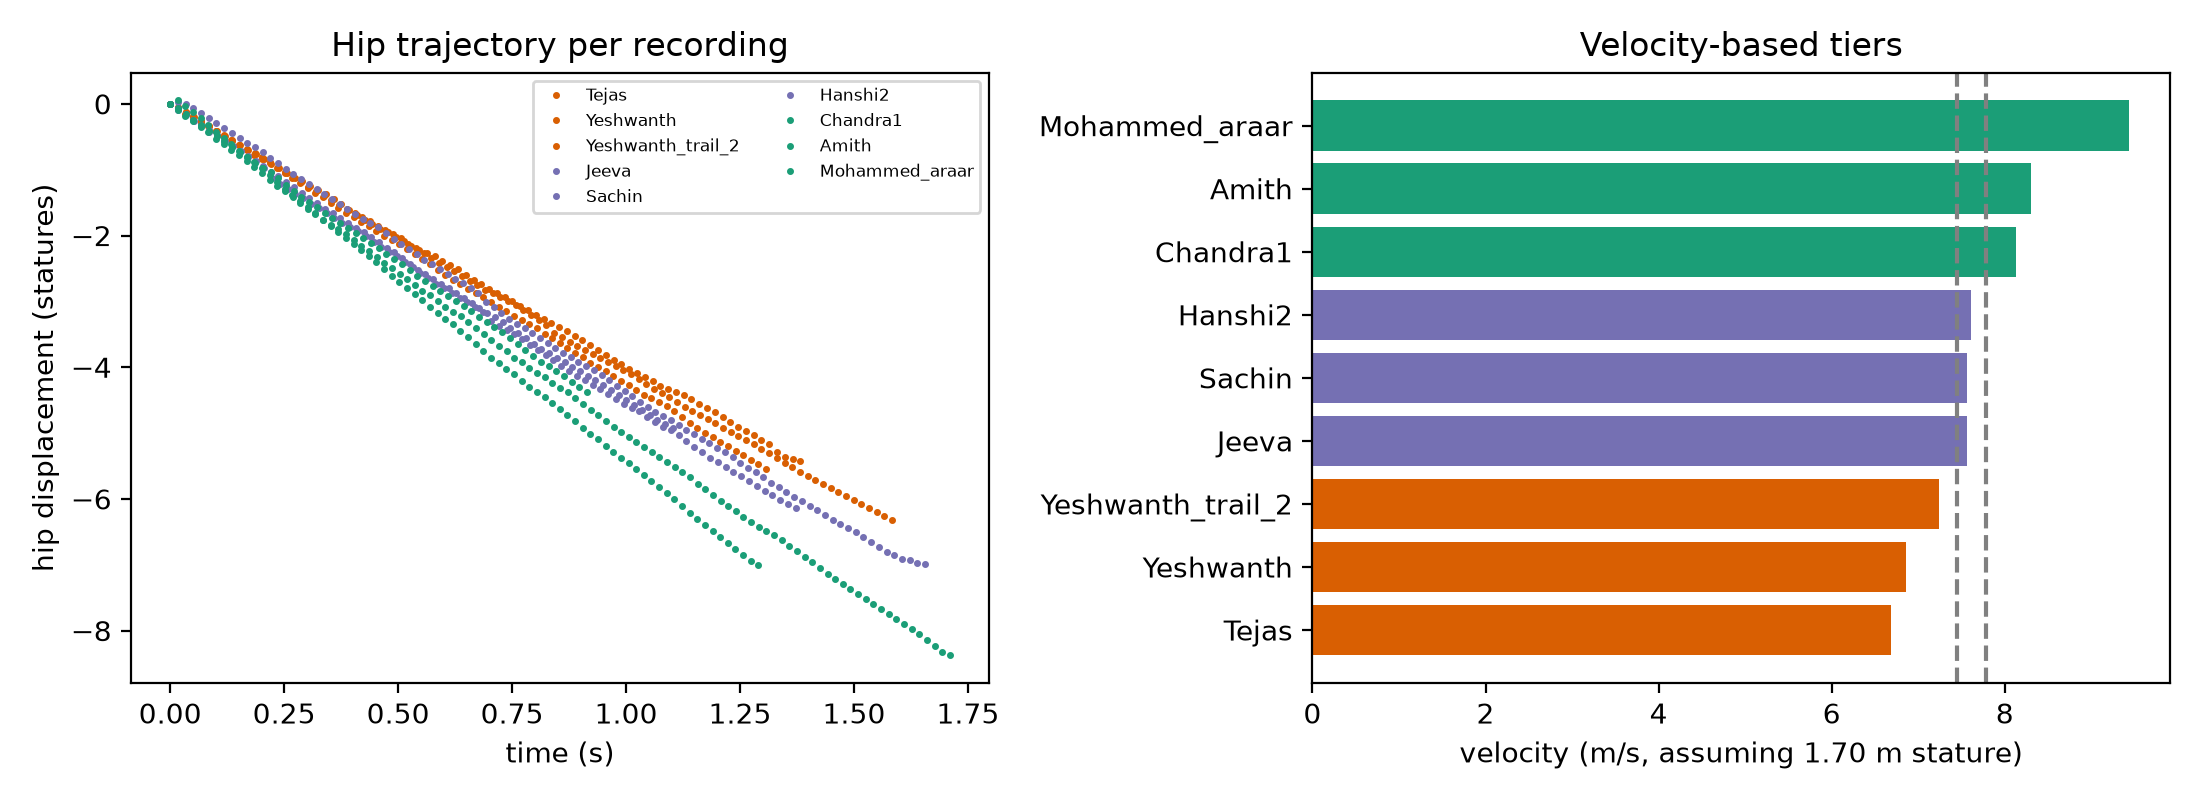
\includegraphics[width=\columnwidth]{figures/speed_labels.png}
\caption{Velocity labels. Left: hip trajectories (statures) per recording; right: measured velocity and tertile thresholds.}
\label{fig:labels}
\end{figure}

\begin{table}[t]
\caption{Recordings, measured velocity $v$ and automatic quality gate. Athletes are anonymised. Tier: B/I/E = Beginner/Intermediate/Elite (thresholds 7.45 and 7.79\,m/s; 1.70\,m stature assumed).}
\label{tab:data}
\centering\footnotesize
\setlength{\tabcolsep}{4pt}
\begin{tabular}{lccccl}
\toprule
Rec. & $v$ (m/s) & Tier & Step (Hz) & GCT (ms) & Gate\\
\midrule
A5 & 9.44 & E & 4.59 & 70 & pass\\
A1 & 8.30 & E & 3.98 & 103 & pass\\
A2 & 8.14 & E & 3.94 & 89 & fail\\
A3 & 7.61 & I & 4.07 & 98 & pass\\
A6 & 7.56 & I & 3.82 & 101 & pass\\
A4 & 7.56 & I & 3.24 & 117 & fail\\
A8 trial 2 & 7.24 & B & 4.26 & 92 & pass\\
A8 trial 1 & 6.86 & B & 4.24 & 112 & pass\\
A7 & 6.68 & B & 3.78 & 85 & pass\\
\bottomrule
\end{tabular}
\end{table}

\subsection{Features}
Nineteen features are extracted per recording: nine from video (mean knee and hip angles, knee and hip symmetry indices $|X_R-X_L|/\bar{X}\times100\%$, trunk lean, vertical hip oscillation in statures, step frequency, ground contact time (GCT) and duty factor) and ten from the IMU (peak, mean and SD of acceleration and angular-velocity magnitude, RMS jerk, arm-swing frequency from a Welch PSD~\cite{welch1967}, and SPARC smoothness~\cite{balasubramanian2015}). A planted foot is stationary in the world frame, so stance is detected when the slower ankle's horizontal speed falls below $0.4\,v$ ($v$ = running speed); this threshold yields physiological step rates (3.2--4.6\,Hz) and GCT (70--117\,ms) on all clips and was not tuned on accuracy. Stride length, clip duration and frame count are excluded: the first is algebraically velocity over step rate (label leakage) and the others depend on how a clip was trimmed.

\section{Video--IMU Integration}\label{sec:integration}
The phone and watch clocks are independent. The IMU segment used is the highest-intensity window whose length equals the time the runner is tracked in the video; accelerometer and gyroscope streams are merged by nearest timestamp (20\,ms tolerance), and fusion is early (feature-level concatenation after per-fold standardisation). Integration is validated rather than assumed (Fig.~\ref{fig:sync}):
\emph{(i) clock consistency:} for 7 of 9 recordings the video creation time follows the watch's last sample by 1.6--5.7\,s (median 2.4\,s), whereas two files differ by $-102$\,s and $-422$\,s, i.e.\ they were recorded during another run;
\emph{(ii) cadence agreement} on the seven consistent recordings: video wrist-swing stride frequency versus the watch gyroscope gives MAE 0.073\,Hz, bias $-0.05$\,Hz, $r=0.95$;
\emph{(iii) waveform agreement:} the cross-correlation between video wrist velocity and the dominant gyroscope axis has $|r|$ of 0.51--0.94 (median 0.76).
These checks run automatically as a data-quality gate (Section~\ref{sec:mlops}), which quarantined both mismatched files without manual inspection.

\begin{figure}[t]
\centering
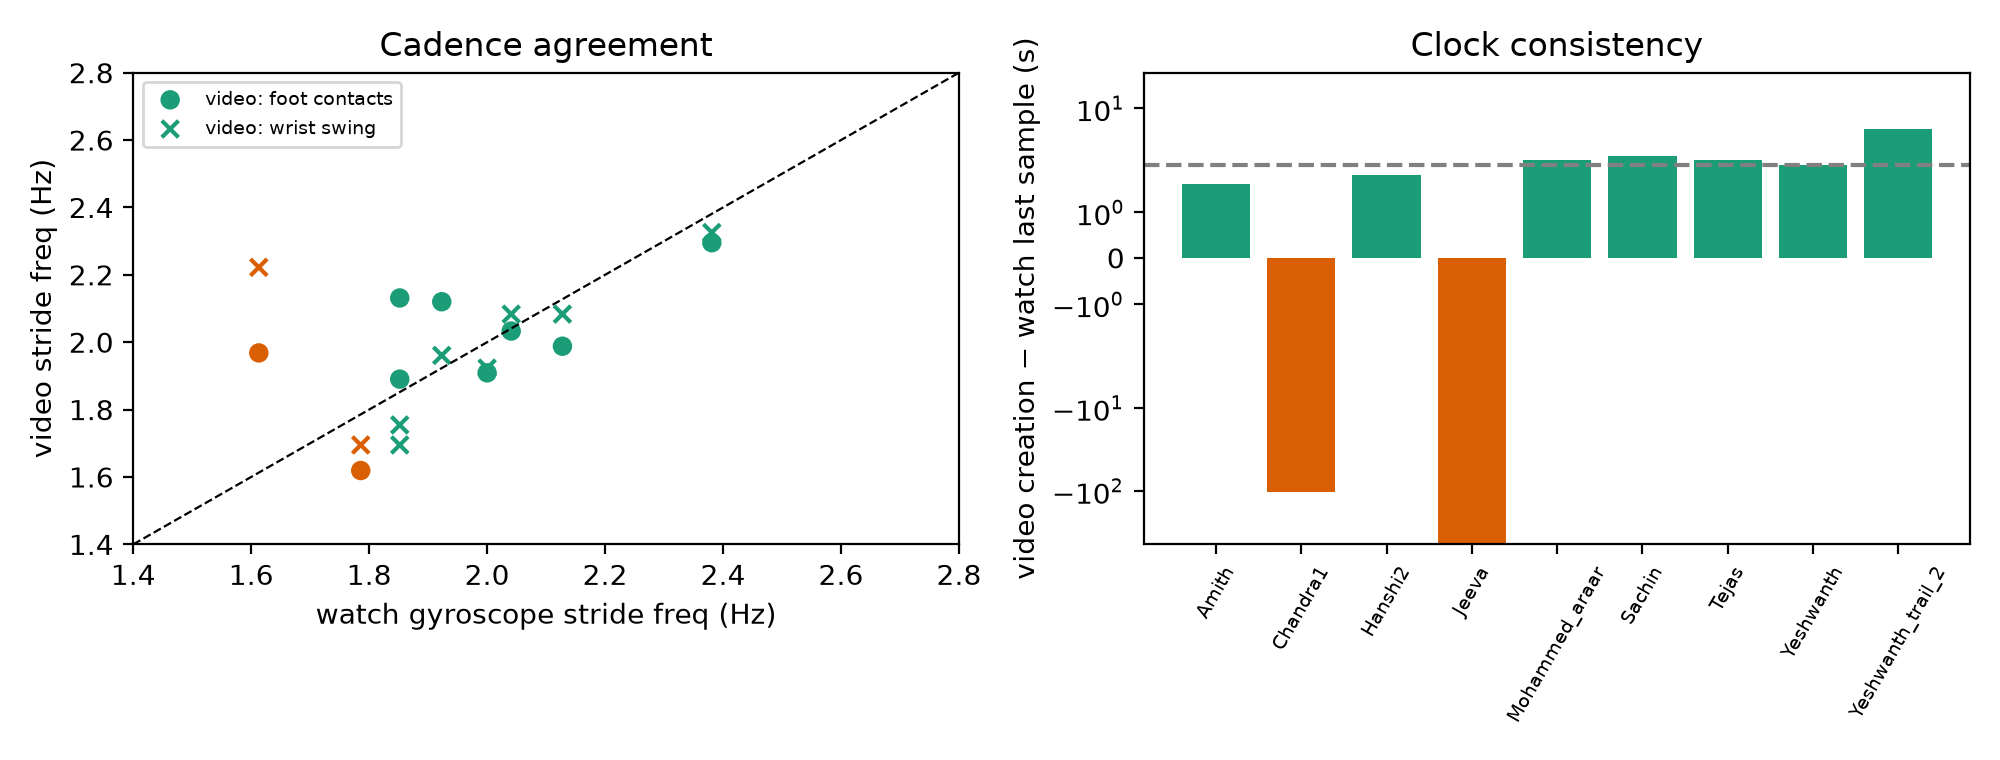
\includegraphics[width=\columnwidth]{figures/sync_validation.png}
\caption{Video--watch integration. Left: stride frequency from video vs.\ watch gyroscope (orange: mismatched files). Right: video--watch clock offset per recording.}
\label{fig:sync}
\end{figure}

\section{MLOps System}\label{sec:mlops}
\begin{figure}[t]
\centering
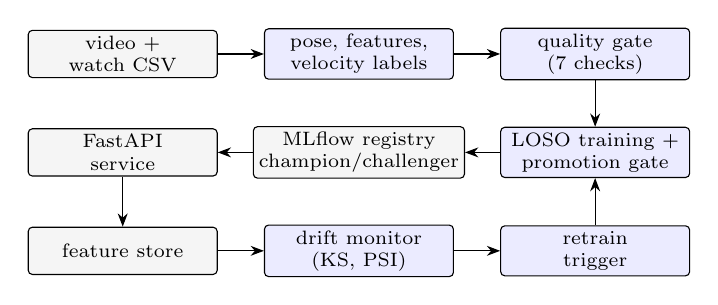
\begin{tikzpicture}[font=\scriptsize, >=Stealth,
 b/.style={draw, rounded corners=1.5pt, minimum height=6mm, minimum width=24mm, inner sep=2pt, align=center, fill=gray!8},
 d/.style={draw, rounded corners=1.5pt, minimum height=6mm, minimum width=24mm, inner sep=2pt, align=center, fill=blue!8}]
\node[b] (raw) at (0,0) {video +\\watch CSV};
\node[d] (feat) at (3.0,0) {pose, features,\\velocity labels};
\node[d] (qa) at (6.0,0) {quality gate\\(7 checks)};
\node[b] (api) at (0,-1.25) {FastAPI\\service};
\node[b] (reg) at (3.0,-1.25) {MLflow registry\\champion/challenger};
\node[d] (tr) at (6.0,-1.25) {LOSO training +\\promotion gate};
\node[b] (fs) at (0,-2.5) {feature store};
\node[d] (mon) at (3.0,-2.5) {drift monitor\\(KS, PSI)};
\node[d] (rt) at (6.0,-2.5) {retrain\\trigger};
\draw[->] (raw)--(feat); \draw[->] (feat)--(qa); \draw[->] (qa)--(tr);
\draw[->] (tr)--(reg); \draw[->] (reg)--(api);
\draw[->] (api)--(fs); \draw[->] (fs)--(mon); \draw[->] (mon)--(rt); \draw[->] (rt)--(tr);
\end{tikzpicture}
\caption{Pipeline. Blue: DVC-versioned batch stages and monitoring; the service serves only the registry \texttt{champion}.}
\label{fig:arch}
\end{figure}

\textbf{Versioning and tracking.} A DVC pipeline (pose $\rightarrow$ features $\rightarrow$ quality gate $\rightarrow$ training) records a hash of the raw data; every MLflow~\cite{zaharia2018} run logs the git commit, data hash, parameters, metrics and evaluation report. All settings live in one parameter file.
\textbf{Data-quality gate.} Seven checks quarantine a recording instead of silently training on it: frame rate ($\geq50$\,fps, because phones record variable 58--60\,fps and 30\,fps footage makes contact features unmeasurable), IMU rate (90--110\,Hz), runner-track fit ($R^2\geq0.99$), tracked frames ($\geq40$), finite features, video--IMU cadence agreement ($\leq0.3$\,Hz) and cohort clock consistency ($\leq5$\,s from the median). The thresholds were set after inspecting these nine recordings and need re-validation on new data. The gate quarantines athlete A2 (cadence 0.48\,Hz off, clock deviation $-104$\,s) and A4 (clock deviation $-424$\,s); seven recordings (six athletes) remain.
\textbf{Promotion gate.} Six candidates (video, IMU or fused features; logistic regression or random forest, with augmentation) are evaluated by leave-one-subject-out (LOSO) cross-validation; the best by macro-F1 is the challenger. A challenger is promoted only if its permutation $p$-value is below 0.05 and its macro-F1 is not below the champion's. The $p$-value uses the maximum statistic over all candidates, which accounts for the selection~\cite{phipson2010}. The first model is registered as \emph{provisional} so the service has something to serve, and the API labels it as such.
The gate is deterministic: (1)~if the training set has fewer than two recordings in a tier or fewer than five athletes, no model is trained and the reason is logged; (2)~otherwise the best candidate's LOSO macro-F1 and max-statistic permutation $p$ are computed; (3)~with no champion, the model is registered as provisional; (4)~with a champion, the challenger is refused if $p\geq0.05$ or its macro-F1 is below the champion's; (5)~every outcome is logged to MLflow and the retraining log. Its known limitation is that it compares macro-F1 across models evaluated on different cohorts, which is only approximately like-for-like.

\textbf{Serving.} A FastAPI service (\texttt{/predict}, \texttt{/health}, \texttt{/metrics}, \texttt{/drift}) in a 1.5\,GB Docker image loads the champion, hot-reloads it on promotion, returns the measured velocity as the primary result and the model's tier flagged as provisional, and logs every request to a feature store. A worker container runs the drift monitor and retraining loop. A Streamlit app is a thin client of the API.
\textbf{Tests.} 43 automated tests (about 9\,s) cover velocity recovery, leakage, each quality rule, drift false-alarm rate and power, the promotion gate, registry restore and the API contract; a regression test checks that the package reproduces the validated features to $10^{-6}$.

\begin{table}[t]
\caption{Automatic data-quality gate: rule, observed range over the nine recordings, and failures.}
\label{tab:qa}
\centering\footnotesize
\setlength{\tabcolsep}{3pt}
\begin{tabular}{@{}llcc@{}}
\toprule
Check & Rule & Observed & Fail\\
\midrule
Video frame rate (fps) & $\geq50$ & 58.3--59.7 & 0\\
IMU rate (Hz) & 90--110 & 99.3--99.6 & 0\\
Runner-track fit $R^2$ & $\geq0.99$ & 0.998--1.000 & 0\\
Tracked frames & $\geq40$ & 55--103 & 0\\
Features finite & all 19 & all & 0\\
Video--IMU cadence diff.\ (Hz) & $\leq0.3$ & 0.001--0.479 & 1\\
Clock offset dev.\ from median (s) & $\leq5$ & $-424$--3.6 & 2\\
\bottomrule
\end{tabular}
\end{table}

\section{Classification Results}\label{sec:results}
\subsection{Protocol}
Evaluation is subject-independent: LOSO cross-validation (eight folds; both trials of the repeated athlete are always held out together). In each fold, only on the training athletes, a standard scaler is fitted and the training set is optionally augmented to 300 samples per class (Gaussian jitter at 5\% of the feature SD plus same-class interpolation). The held-out athlete therefore never influences scaling, augmentation or early stopping; a unit test confirms that a held-out athlete's prediction does not change with its own label. Classifiers are logistic regression ($C=1$), an RBF-SVM ($C=1$), a random forest (100 trees, depth 5) and an MLP (128--64--32 ReLU, batch normalisation, dropout 0.4/0.3/0.2, L2 $10^{-3}$, Adam $10^{-3}$, at most 100 epochs, early stopping with patience 10; five seeds). We report accuracy, macro precision, recall and F1 over the nine pooled out-of-fold predictions, subject-level bootstrap 95\% CIs (2000 resamples) and label-permutation $p$-values (200 permutations).

\subsection{Results}
\begin{table}[t]
\caption{LOSO results (chance 33\%). Best model per modality by macro-F1. $p$: permutation test (not selection-corrected).}
\label{tab:res}
\centering\small
\setlength{\tabcolsep}{3pt}
\begin{tabular}{llccccc}
\toprule
Modality & Model & Acc.\ (\%) & P & R & F1 & 95\% CI / $p$ \\
\midrule
\multicolumn{7}{l}{\emph{All recordings: 8 athletes, 9 trials}}\\
Video & LogReg+aug & 33.3 & .33 & .33 & .32 & 9--75 / .44\\
IMU & LogReg+aug & 55.6 & .42 & .56 & .48 & 25--88 / .16\\
Fused & MLP & 28.9$\pm$16.9 & .23 & .29 & .24 & 13--89 / --\\
\multicolumn{7}{l}{\emph{Watch files verified: 6 athletes, 7 trials}}\\
Video & SVM+aug & 28.6 & .33 & .33 & .33 & 0--67 / .44\\
IMU & RF+aug & 57.1 & .50 & .56 & .52 & 25--86 / .10\\
Fused & RF+aug & 14.3 & .08 & .11 & .10 & 0--33 / .70\\
\bottomrule
\end{tabular}
\end{table}

\begin{figure}[t]
\centering
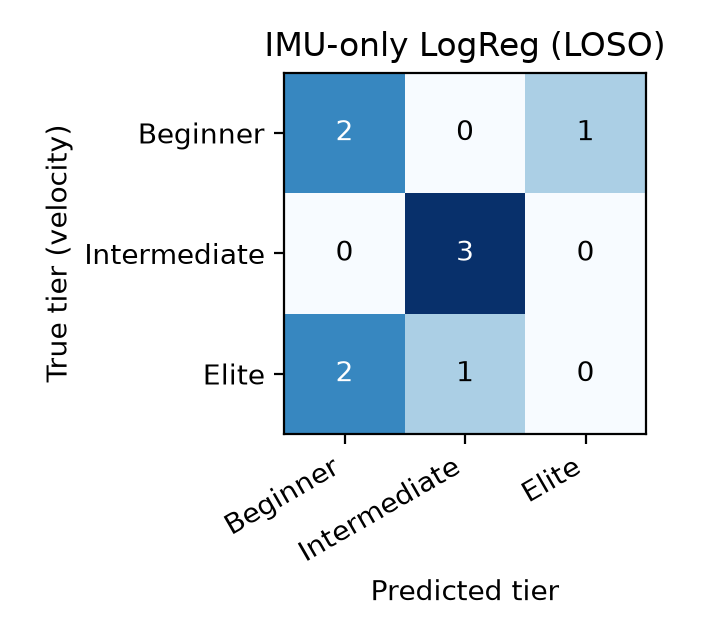
\includegraphics[width=0.49\columnwidth]{figures/confusion_IMU-only_LogReg_best.png}\hfill
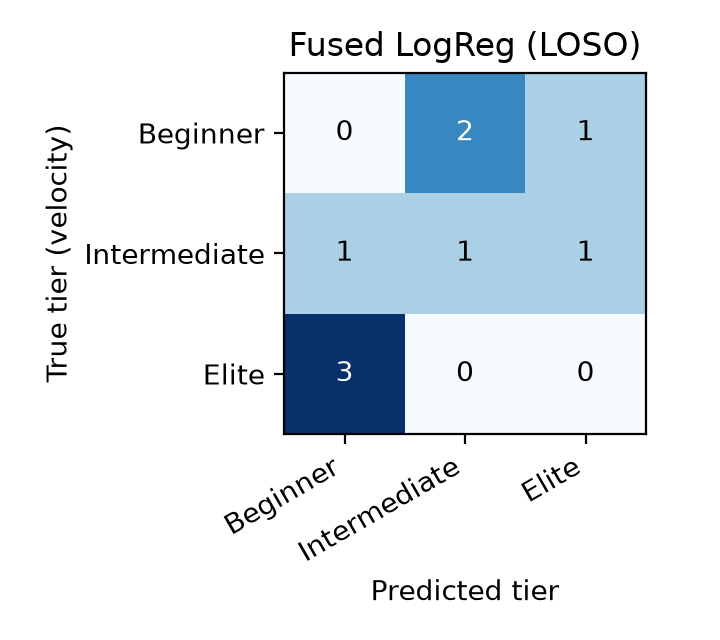
\includegraphics[width=0.49\columnwidth]{figures/confusion_Fused_LogReg_best.png}
\caption{Pooled LOSO confusion matrices (9 recordings): IMU-only logistic regression (left) and fused logistic regression (right).}
\label{fig:cm}
\end{figure}

Table~\ref{tab:res} and Fig.~\ref{fig:cm} give the leakage-free results. No configuration is significantly above chance (smallest $p=0.10$), several score below chance (a known artefact of leave-one-out with classes of three samples), and early fusion does not outperform the single modalities. A LOSO ridge regression of velocity does not beat a training-mean predictor either (MAE 0.80--0.88 vs.\ 0.71\,m/s). The model deployed by the pipeline, selected among six candidates on seven verified recordings with selection-corrected $p$, scores 28.6\% (macro-F1 0.24, $p=0.67$) and is therefore served as provisional. Descriptively, GCT correlates negatively with velocity ($r=-0.52$) and step frequency positively ($r=0.40$), consistent with~\cite{weyand2000}, but $n=9$ is too small for inference.

\emph{Relation to earlier accuracies.} The earlier version of this system reported 82--100\%. Those figures came from (a) K-Means labels computed on the input features themselves and (b) synthetic samples generated from all athletes \emph{before} the train/test split, so every test athlete had near-copies in the training set. We report this because both pitfalls are common in small-sample sports analytics.

\section{Latency}\label{sec:latency}
\begin{table}[t]
\caption{Measured per-stage latency, median (p95 where given). Apple M5, MediaPipe 0.10.9. $^\dagger$Deployed configuration (pose complexity 1).}
\label{tab:lat}
\centering\small
\setlength{\tabcolsep}{4pt}
\begin{tabular}{lcc}
\toprule
Stage & All cores & E-cores only\\
\midrule
Video decode, per frame & 1.4\,ms & 10.6\,ms\\
Pose lite, per frame & 7.1 (13.0)\,ms & 45.8 (75.8)\,ms\\
Pose full$^\dagger$, per frame & 11.5 (17.9)\,ms & 61.3 (114)\,ms\\
Pose heavy, per frame & 49.3 (56.3)\,ms & 212 (273)\,ms\\
Features, per sprint & 8.1\,ms & 49.9\,ms\\
MLP, Keras \texttt{predict} & 14.5\,ms & 95\,ms\\
MLP, TFLite (52\,KB) & 1.1\,$\mu$s & 9.3\,$\mu$s\\
End-to-end, per clip$^\dagger$ & 2.1\,s & 12.7\,s\\
\bottomrule
\end{tabular}
\end{table}
Pose estimation dominates (Table~\ref{tab:lat}); once exported to TFLite the classifier costs microseconds, and the Keras \texttt{predict} figure (14.5--95\,ms) is framework overhead, not model compute. Through the Docker API a full request (upload, pose, features, classifier) has a median of 2.1\,s for one user. On-phone execution was not measured and is future work.

\section{Drift Monitoring and Retraining}\label{sec:drift}
\emph{Thresholds.} Each feature is tested against the training reference with a two-sample Kolmogorov--Smirnov test~\cite{massey1951} at the Bonferroni-corrected $\alpha=0.05/19=0.0026$, which bounds the family-wise false-alarm rate at 5\% (a unit test asserts $\leq10\%$ over 300 null windows); the population stability index is a secondary signal~\cite{gama2014}. A Monte-Carlo power analysis (Fig.~\ref{fig:power}) shows that a 1-SD shift in one feature is detected with 84\% probability only with a reference of $\geq100$ and a window of $\geq30$; with our 9-sample reference power never exceeds 29\%. Alarms are therefore \emph{armed} only above those sizes and reported as informational below them; our reference has 7 recordings, so no alarm is armed today. Retraining is triggered by an armed alarm, every three new quality-passed recordings (a parameter; low-risk because of the promotion gate), or manually.

\begin{figure*}[t]
\centering
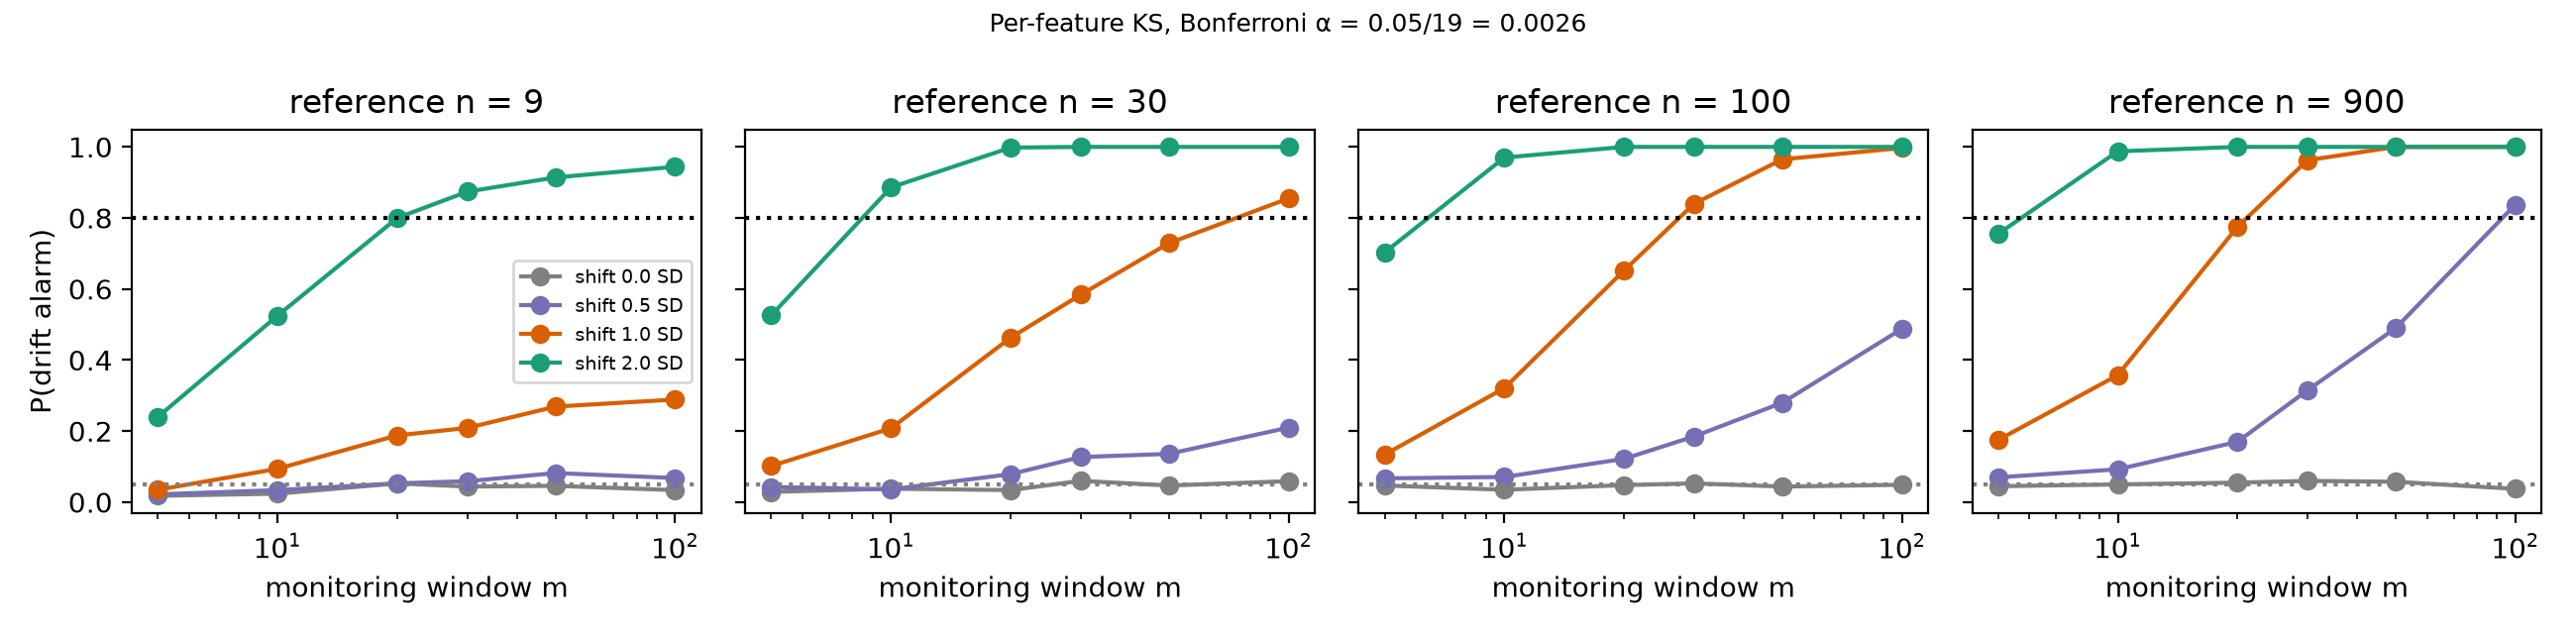
\includegraphics[width=0.92\textwidth]{figures/drift_power.png}
\caption{Detection probability of the per-feature KS monitor versus window size for reference sets of 9, 30, 100 and 900 samples.}
\label{fig:power}
\end{figure*}

\emph{Device-shift replay.} Seven real clips were replayed through the API with simulated device changes. Unmodified clips raise no alarm; a 50\,Hz watch is rejected by the quality gate in 7/7 cases and never reaches the monitor; a $\times1.5$ accelerometer gain raises an informational alarm on peak acceleration, acceleration SD and RMS jerk ($p=0.00058$ each). A 30\,fps camera makes contact features unmeasurable, so 60\,fps capture is a hard requirement.
\emph{Changing population.} Replaying the nine recordings in capture order from a cold start, two are quarantined, a first (provisional, $p=0.099$) model appears at the 8th arrival, and the retrained challenger at the 9th is refused ($p=0.65$, macro-F1 0.24 vs.\ 0.56). The loop and gate work, but \textbf{an accuracy benefit from retraining could not be demonstrated} at this sample size.

\section{Throughput, Fault Tolerance and Availability}\label{sec:ops}
\begin{table}[t]
\caption{Load test (Docker, 10-core node; real 2--3\,s clip incl.\ upload; 45\,s per row). 214 requests, 0 failures.}
\label{tab:load}
\centering\small
\begin{tabular}{ccccc}
\toprule
Workers & Users & Req/s & Median & p95\\
\midrule
1 & 1 & 0.48 & 2.1\,s & 2.1\,s\\
1 & 4 & 1.21 & 3.3\,s & 3.5\,s\\
2 & 4 & 1.14 & 3.5\,s & 3.6\,s\\
4 & 4 & 1.04 & 3.8\,s & 4.2\,s\\
4 & 8 & 1.11 & 6.5\,s & 7.0\,s\\
\bottomrule
\end{tabular}
\end{table}
Throughput saturates near 1.2 clips/s ($\approx$70/min) irrespective of worker count (Table~\ref{tab:load}) because MediaPipe already parallelises within a request; scaling beyond one node was not tested. In fault tests, killing one of two workers under a 100\,ms health probe caused no failed probe and a replacement within 0.03\,s; SIGKILL of the server process was recovered by the container restart policy in 0.9--1.0\,s, and a container restart took 3.8--3.9\,s (three trials each). A fault-free health probe succeeded 60/60 times over five minutes. A window this short cannot support an availability figure near 99.5\%, so we make no such claim.

\section{Reproducibility}
Table~\ref{tab:repro} lists the environment. \texttt{dvc repro} rebuilds the pipeline from raw recordings, every number here is regenerated by the released scripts, and the tests run without the recordings. Pose features differ slightly between macOS and the Linux container (e.g.\ 8.30 vs.\ 8.32\,m/s), so the platform is stated with each result.
\begin{table}[t]
\caption{Reproducibility settings.}\label{tab:repro}
\centering\small
\setlength{\tabcolsep}{3pt}
\begin{tabular}{@{}lp{0.74\columnwidth}@{}}
\toprule
Camera & smartphone, 1080p HEVC, 60\,fps, tripod\\
Watch & Galaxy Watch4 Classic (left wrist), 99.3--99.6\,Hz\\
Compute & Apple M5 (10 cores), 16\,GB, macOS 27.0.1; Docker VM 10 CPUs, 8\,GB\\
Software & Python 3.11.17, MediaPipe 0.10.9, scikit-learn 1.7.2, NumPy 1.26.4, pandas 2.3.3, SciPy 1.17.1, OpenCV 4.11, TensorFlow 2.18.1, MLflow 3.5.1, DVC 3.67.1, FastAPI 0.162.2\\
Settings & seed 42 (MLP 42--46); pose complexity 1; all in \texttt{params.yaml}\\
\bottomrule
\end{tabular}
\end{table}

\section{Discussion}
\emph{What the data can and cannot say.} The measurement layer is validated: velocity labels fit every trajectory almost perfectly, video and watch agree on cadence, and mismatched files are caught automatically. The prediction layer is not: with eight athletes, the standardisation of many weakly informative features lets a classifier fit spurious patterns in small training folds, which is the same effect that makes fusion worse than a single modality in Table~\ref{tab:res}. For this reason the service reports the measured velocity as its primary output and the model tier only as provisional.
\emph{Earlier UTD-MHAD experiment.} The earlier version reported 87\% three-class fusion accuracy on UTD-MHAD jogging, with tiers defined as terciles of a video feature (mean hip angle). Re-running that experiment gives 62.5\% and, because the label is derived from an input, it is not a valid skill test; we withdraw it. As a measurement check we also compared video and thigh-IMU stride frequency on its 32 jogging-in-place trials and found no agreement (MAE 0.54\,Hz, $r=-0.02$), so we make no claim that our cadence method transfers to that activity.
\emph{Practical implication.} Because labelling is automatic, every new recording that passes the gate is both a prediction request and a labelled training example; reaching the 100-recording milestone needs no annotation effort, only data collection, which is what the monitor and promotion gate are designed to make safe.

\section{Limitations}\label{sec:limits}
(1) Eight athletes from one session: the classification study is a pilot and supports no claim of generalisation. (2) Tiers are cohort-relative tertiles; absolute velocity assumes a 1.70\,m stature ($\approx\pm5\%$ per 8.5\,cm). (3) 2-D pose from one side view; joint-angle accuracy was not validated against motion capture. (4) Quality-gate thresholds were set on these recordings. (5) Only the part of the fly zone inside the field of view (0.9--1.7\,s) is analysed. (6) Latency was measured on one laptop CPU, not on phones; throughput on one node. (7) Retraining benefit and availability over long periods remain unmeasured.

\section{Conclusion}
We presented a reproducible smartphone-plus-smartwatch sprint-analysis pipeline with an objective velocity label, a validated and automatically checked video--IMU integration, a promotion-gated registry, drift monitoring justified by a power analysis, and measured latency, throughput and fault-tolerance. A leakage-free pilot showed that three-tier skill classification is not yet reliable with eight athletes, and that earlier accuracies were artefacts of label circularity and augmentation leakage. At least 100 labelled recordings are needed before drift alarms can be armed; because labelling is automatic, routine use can reach that milestone cheaply, which is the next step.

\section*{Acknowledgment}
The authors thank Dr.~Bahubali Shiragapur and Dr.~Puneeth~N for guidance and mentorship, the Department of Physical Education at Dayananda Sagar University for facility access and athlete recruitment support, and all participating athletes.

\begin{thebibliography}{00}
\bibitem{weyand2000} P.~G. Weyand, D.~B. Sternlight, M.~J. Bellizzi, and S.~Wright, ``Faster top running speeds are achieved with greater ground forces not more rapid leg movements,'' \emph{J. Appl. Physiol.}, vol.~89, no.~5, pp. 1991--1999, 2000.
\bibitem{colyer2018} S.~L. Colyer, M.~Evans, D.~P. Cosker, and A.~I.~T. Salo, ``A review of the evolution of vision-based motion analysis and the integration of advanced computer vision methods towards developing a markerless system,'' \emph{Sports Med.\ Open}, vol.~4, art.~24, 2018.
\bibitem{bazarevsky2020} V.~Bazarevsky \emph{et al.}, ``BlazePose: On-device real-time body pose tracking,'' arXiv:2006.10204, 2020.
\bibitem{cao2021} Z.~Cao, G.~Hidalgo, T.~Simon, S.-E. Wei, and Y.~Sheikh, ``OpenPose: Realtime multi-person 2D pose estimation using part affinity fields,'' \emph{IEEE Trans.\ Pattern Anal.\ Mach.\ Intell.}, vol.~43, no.~1, pp. 172--186, 2021.
\bibitem{kidzinski2020} {\L}.~Kidzi{\'n}ski \emph{et al.}, ``Deep neural networks enable quantitative movement analysis using single-camera videos,'' \emph{Nat.\ Commun.}, vol.~11, art.~4054, 2020.
\bibitem{sculley2015} D.~Sculley \emph{et al.}, ``Hidden technical debt in machine learning systems,'' in \emph{Proc.\ NeurIPS}, 2015.
\bibitem{sen1968} P.~K. Sen, ``Estimates of the regression coefficient based on Kendall's tau,'' \emph{J. Am.\ Stat.\ Assoc.}, vol.~63, no.~324, pp. 1379--1389, 1968.
\bibitem{drillis1966} R.~Drillis and R.~Contini, ``Body segment parameters,'' New York Univ., School of Eng.\ and Science, Tech.\ Rep.\ 1166-03, 1966.
\bibitem{welch1967} P.~D. Welch, ``The use of fast Fourier transform for the estimation of power spectra,'' \emph{IEEE Trans.\ Audio Electroacoust.}, vol.~15, no.~2, pp. 70--73, 1967.
\bibitem{balasubramanian2015} S.~Balasubramanian, A.~Melendez-Calderon, A.~Roby-Brami, and E.~Burdet, ``On the analysis of movement smoothness,'' \emph{J. NeuroEng.\ Rehabil.}, vol.~12, art.~112, 2015.
\bibitem{zaharia2018} M.~Zaharia \emph{et al.}, ``Accelerating the machine learning lifecycle with MLflow,'' \emph{IEEE Data Eng.\ Bull.}, vol.~41, no.~4, pp. 39--45, 2018.
\bibitem{phipson2010} B.~Phipson and G.~K. Smyth, ``Permutation $p$-values should never be zero,'' \emph{Stat.\ Appl.\ Genet.\ Mol.\ Biol.}, vol.~9, no.~1, art.~39, 2010.
\bibitem{massey1951} F.~J. Massey, ``The Kolmogorov--Smirnov test for goodness of fit,'' \emph{J. Am.\ Stat.\ Assoc.}, vol.~46, no.~253, pp. 68--78, 1951.
\bibitem{gama2014} J.~Gama, I.~{\v Z}liobait{\.e}, A.~Bifet, M.~Pechenizkiy, and A.~Bouchachia, ``A survey on concept drift adaptation,'' \emph{ACM Comput.\ Surv.}, vol.~46, no.~4, art.~44, 2014.
\end{thebibliography}
\end{document}
